%% Preamble
\documentclass{beamer}
\usetheme{Warsaw}
\usepackage{url}
\usepackage{xcolor}

\AtBeginSection[]
{
	\begin{frame}
		\frametitle{Table of Contents}
		\tableofcontents[currentsection]
	\end{frame}
}

\title{Parallel computing in Julia}
\author{Jasper Boomer}
\titlegraphic{
\includegraphics[width=.3\textwidth]{figures/logo.png}}

%% Document
\begin{document}

	\frame{\titlepage}

	\section{Introduction}

	\begin{frame}{Background(1)}
		\begin{quote}
			" We want a language that’s open source, with a liberal license. We want the speed of C with the dynamism of Ruby. We want a language that’s homoiconic, with true macros like Lisp, but with obvious, familiar mathematical notation like Matlab. We want something as usable for general programming as Python, as easy for statistics as R, as natural for string processing as Perl, as powerful for linear algebra as Matlab, as good at gluing programs together as the shell. Something that is dirt simple to learn, yet keeps the most serious hackers happy. We want it interactive and we want it compiled."
		\end{quote}
		Julia developers on "Why we created Julia"
	\end{frame}


	\begin{frame}{Background(2)}
		Julia is: 
		\begin{itemize}
			\item{General purpose high-level dynamic programming language}
			\item{Free \& Open source (MIT licensed)}
			\item{Development started in 2009, v0.1 in 2012}
			\item{Designed for parallelism \& distributed computation}
			\item{Core written in C/C++, STL in Julia}
			\item{JIT Compiled}
			\item{Optimized for speed of calculation}
		\end{itemize}
	\end{frame}

	\begin{frame}{Benchmarks}
		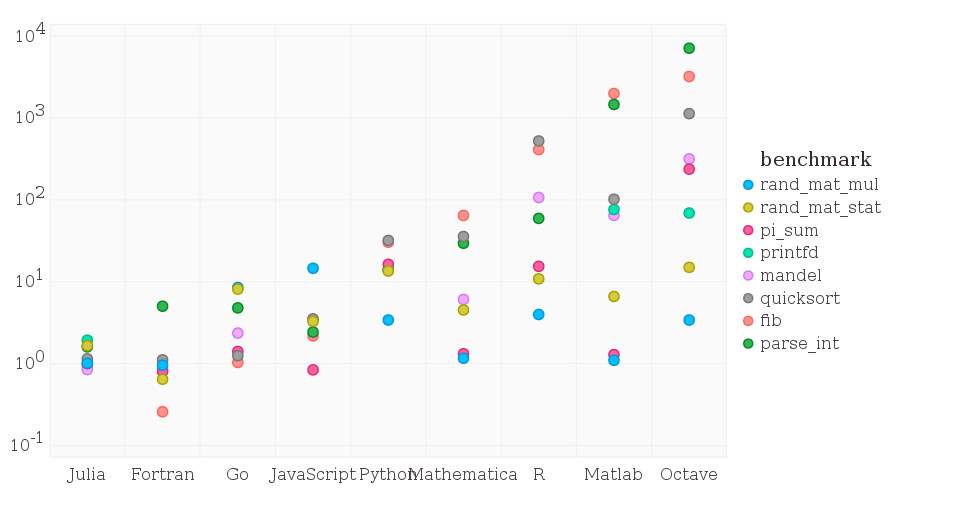
\includegraphics[width=\textwidth]{figures/benchmarks.jpg}
		\footnote{Speed relative to C}
	\end{frame}

	\begin{frame}[fragile]{Some syntax}
		\begin{block}{Examples}
			\begin{semiverbatim}
			julia> [i*2 for i=1:5]   
			[1 4 6 8 10]
			
			julia> function printargs(args...)
			         for a in args
		 	           println(a)
			         end
			       end

			julia> map(x->(x\%3==0), [3 4 12])
			[true, false, true]        
			\end{semiverbatim}
		\end{block}
	\end{frame}

	\begin{frame}[fragile]{Macros}
		Expressions are Julia objects. These can be modified and then run.
		\begin{block}{@time macro}
			\begin{semiverbatim}
			macro time(d::Expr) 
			  local t0 = time()
			  local val = \$d
			  tocal t1 = time()
			  println("elapsed time: ", t1-t0, " seconds")
			  return val
			end

			julia> @time rand(100,100)
			elapsed time 0.00679384 seconds
			100x100 Array\{Float64\}
			\end{semiverbatim}
		\end{block}
	\end{frame}

	\section{Tasks}

	\begin{frame}{Tasks(1)}
		\begin{columns}[c]
			\column{0.5\textwidth}
				\textbf{Functions (Sub-routines)} \\
				Call / Return
				\includegraphics[width = .6\textwidth]{figures/functions.eps}
			\column{0.5\textwidth}
				\textbf{Tasks (Co-routines)} \\
				Yielding to other tasks (saving state) \\
				
\includegraphics[width = .6\textwidth]{figures/tasks.eps}
		\end{columns}
	\end{frame}

	\begin{frame}{Tasks(2)}
		Example: Integrator \\
		\includegraphics[width=.6\textwidth]{figures/integrator.eps}
	\end{frame}	

	\section{Low level parallel Julia}

	\begin{frame}{Parallel implementation in Julia}
		\begin{itemize}
			\item{No native threads (yet?)}
			\item{Uses tasks/coroutines for scheduling}
			\item{Message passing interface for data communication}
			\item{Implementation of message passing is one-sided}
		\end{itemize}
	\end{frame}
	
	\begin{frame}[fragile]{Worker processes}
		\begin{block}{Syntax:}
		\begin{semiverbatim}
			julia -p N [filename]
		\end{semiverbatim}
		\end{block}
		\begin{itemize}
			\item{Launches \verb+N+ worker processes}
			\item{Runs \verb+filename+ or interactive session}
			\item{Workers are numbered $2:N+1$}
			\item{Can run on multiple cores or cluster of computers (specified using a machinefile)}
		\end{itemize}
	\end{frame}

	\begin{frame}[fragile]{Remote calls \& references}
		\begin{block}{Executing statements on specific worker processes}
		\begin{semiverbatim}
		julia -p 2
		julia> r = remotecall(2, sin, pi/4)
		RemoteRef(3,1,2) 

		julia> fetch(r)
		0.7071067811865475

		julia> remotecall\_fetch(2, myid)
		2
		
		julia> @spawn cos(pi/4) 
		RemoteRef(3,1,3)
		\end{semiverbatim}
		\end{block}
	\end{frame}

	\section{MapReduce}

	\begin{frame}[fragile]{Parallel map}
		\begin{block}{Parallel map:}
		\begin{semiverbatim}
			pmap(function, collection)
		\end{semiverbatim}
		\end{block}
		Performs \verb+function+ on \verb+collection+. Uses a 'feeder' task for each worker process to serve data, while waiting for result the task yields to next feeder task until work is complete. 
		\begin{block}{Example: list of expressions}
			\begin{semiverbatim}
				julia> pmap(eval, \{:(4+4), :(4*4), :(7-2), :(6/2)\} )
				[8, 16, 5, 3]
			\end{semiverbatim}
		\end{block}
	\end{frame}

	\begin{frame}[fragile]{MapReduce}
		\begin{columns}
		\column{.7\textwidth}
		\begin{block}{MapReduce macro:}
			\begin{semiverbatim}
				@parallel (reduction) for collection
			\end{semiverbatim}
		\end{block}
		\begin{block}{Example: coin toss}	
		\begin{semiverbatim}
		heads = 
		@parallel (+) for i=1:10000000
		  randbool()
		end
		\end{semiverbatim}
		\end{block}
		\column{.3\textwidth}
		\includegraphics[width = \textwidth]{figures/parallel_map.eps}
		\end{columns}
	\end{frame}

	\begin{frame}{Example}
		Example: \\
		A slice of  $\pi$
		\begin{columns}[c]
			\column{0.5\textwidth}
			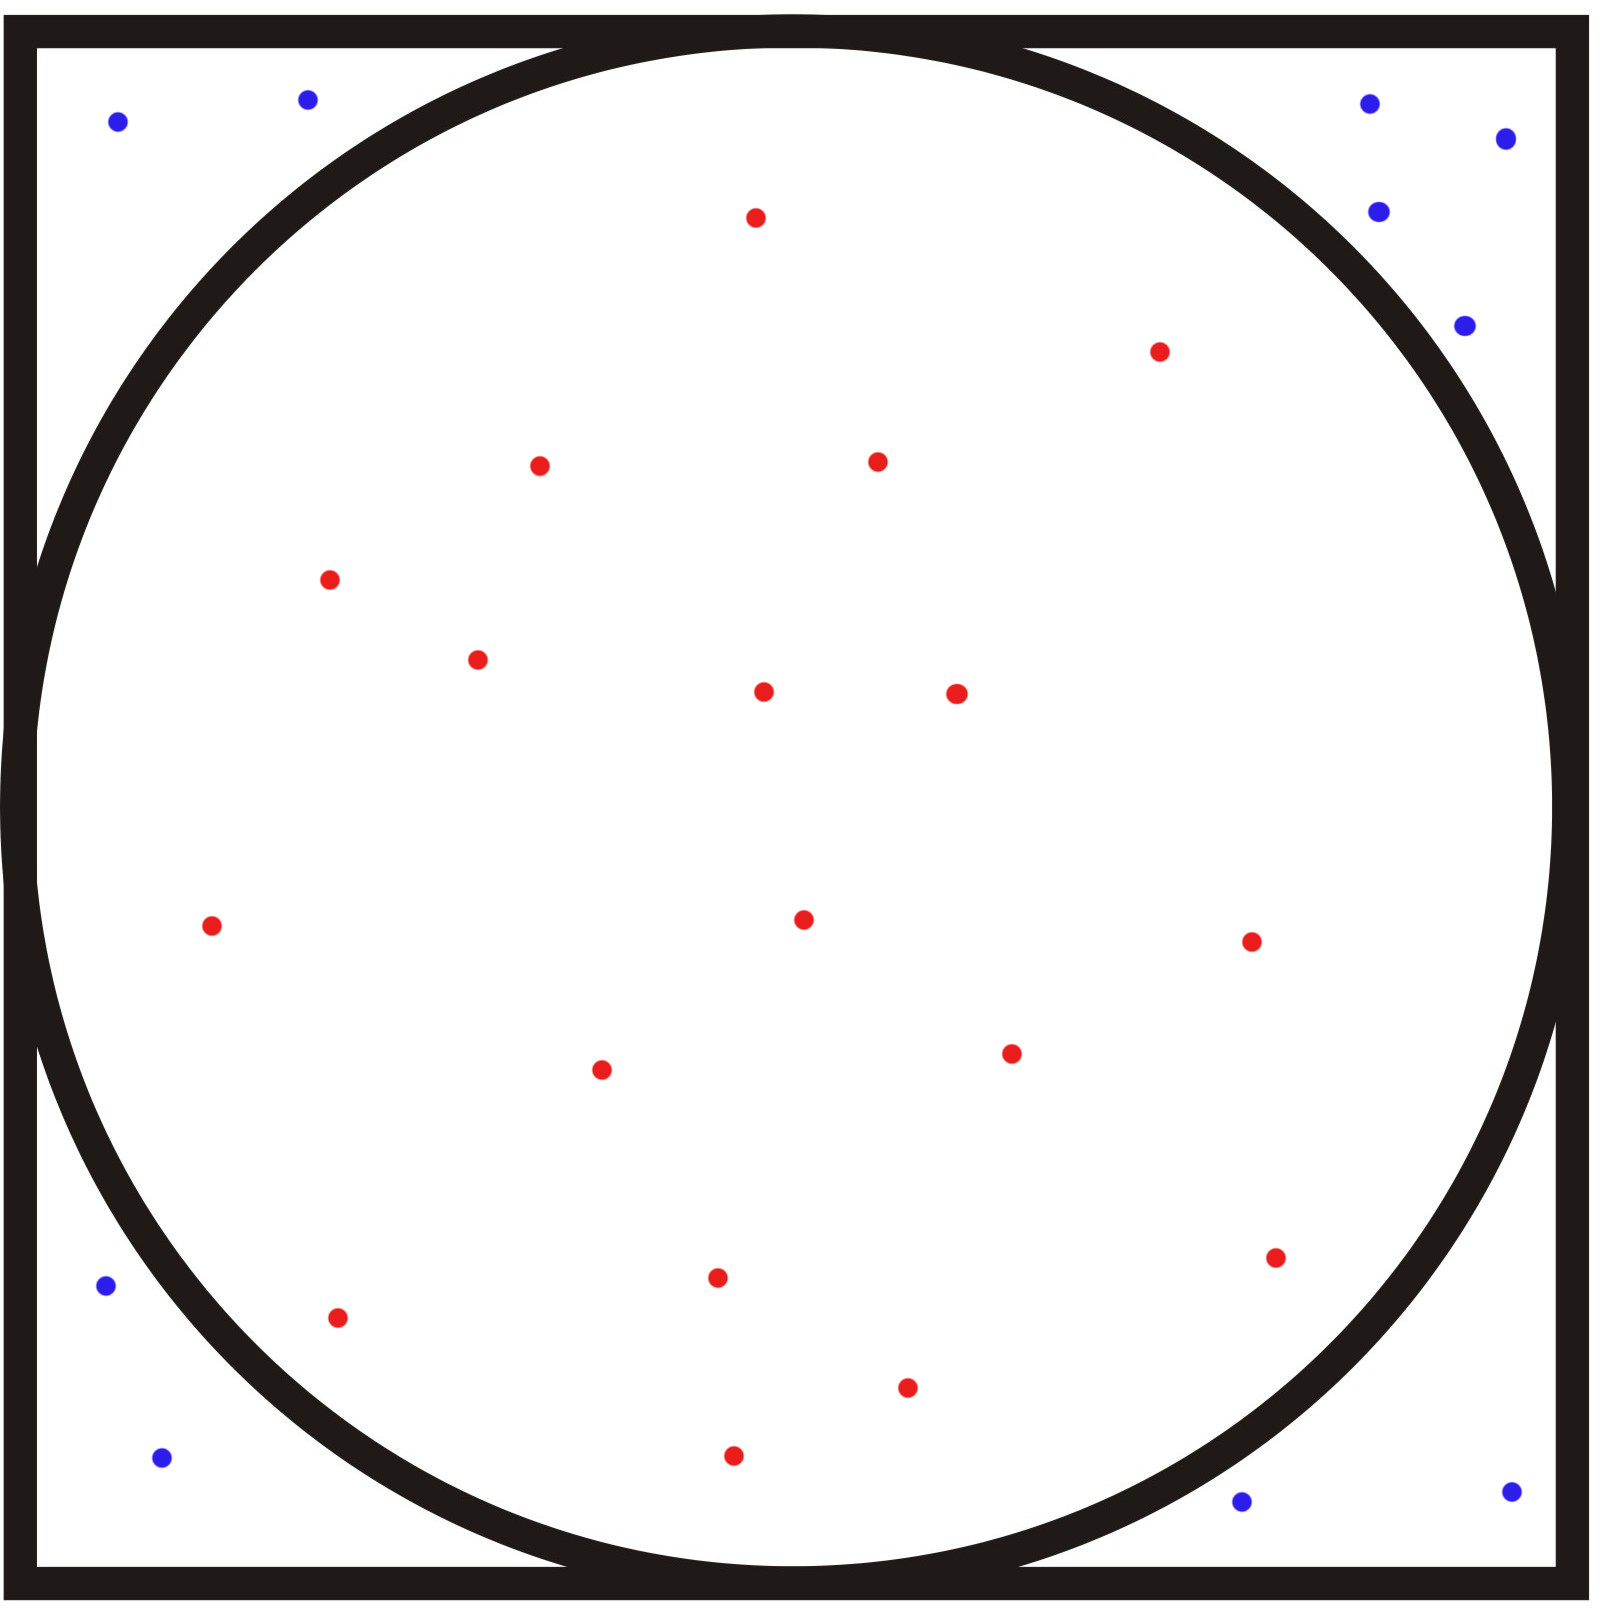
\includegraphics[height=4cm]{figures/square_circle.jpg}
			\column{0.5\textwidth}
			Generate random points from uniform distribution, get $\pi$ from ratio of points in the circle.
			\begin{equation*}
				\begin{array}{rcl}		
					A_{rect} & = & (2r)^2 = 4r^2 \\
					A_{circle} & = & \pi r^2 \\
					\pi & = & 4\frac{A_{circle}}{A_{rect}}
				\end{array}
			\end{equation*}
		\end{columns}
	\end{frame}

	\section{Distributed arrays}
	\begin{frame}[fragile]{Syntax}
    \begin{block}{Constructor:}
		\verb+DArray(init, dims[, procs, dist])+
		\end{block}
		\begin{block}{Example with 8 workers:}
		\begin{semiverbatim}
		julia> d = DArray(I->rand(length(I[1]),length(I[2])),
											(80, 80),  #dimensions
											[2:9],     #worker processes
											[4,2]);	   #distribution
		
		julia> remotecall\_fetch(2,localindexes,d)
		(1:20, 1:40)
		julia> remotecall\_fetch(7,localindexes,d)
		(21:40, 41:80)
		\end{semiverbatim}
		\end{block}
	\end{frame}

	\begin{frame}{Example: Mandelbrot Set}
		\begin{columns}[c]
		\column{.5\textwidth}
			
\includegraphics[height = 4cm]{figures/mandel_zoom.jpg}	
		\column{.5\textwidth}
			\begin{equation*}
			\begin{array}{rcl}
				z\in\mathbb{C}: & & \\
				z_0 & = & z	\\
				z_{n+1} & = & z_n^2 + z
			\end{array}
			\end{equation*}
			Set of $c$ for which orbit of z around 0 remains bounded. Colours indicate escape time.
		\end{columns}
	\end{frame}
	
	\section{Last words}
	
	\begin{frame}{Links}
		\begin{itemize}
			\item{\url{http://julialang.org/}}
			\item{\url{http://learnxinyminutes.com/docs/julia/}}
			\item{\url{https://github.com/jboomer/parallel-julia/}}
			\item{\url{http://www.dabeaz.com/coroutines/}}
		\end{itemize}
	\end{frame}
	
	\section{Questions}

\end{document}
